% --------------------------
% APPENDIX
% --------------------------
\appendix
\clearpage

\chapter{Appendix}

This appendix collects supplementary material to the main text, comprising mathematical derivations, implementation details, additional empirical results, and the code produced for this thesis.

\section{Code}

The code developed for this thesis, including implementations of the affine-inspired encoder-decoder and all simulation and evaluation experiments, is made publicly available at:
\begin{center}
\url{https://github.com/sarasvenstrup/MasterThesis}
\end{center}


\section{Derivatives Used to Derive the Bond-Pricing ODE System}
\label{app:pde_derivatives}

This section derives the maturity and state derivatives of the model-implied bond price required in the bond-pricing PDE.

Define, for notational convenience
\[
\Phi(z,\tau):=A_z(\tau)-B_z(\tau)\,\mathcal{G}(z,\tau),
\qquad\text{such that}\qquad
P(z,\tau)=e^{\Phi(z,\tau)}.
\]

Differentiating with respect to maturity $\tau$ by applying the chain rule gives
\[
\partial_\tau P(z,\tau) = (\partial_\tau \Phi(z, \tau))\,P(z, \tau),
\]
where
\[
\partial_\tau \Phi(z, \tau)
=
\partial_\tau A_z(\tau) - \partial_\tau\!\big(B_z(\tau)\,\mathcal{G}(z,\tau)\big)
=
\partial_\tau A_z(\tau)
-
(\partial_\tau B_z(\tau))\,\mathcal{G}(z,\tau)
-
B_z(\tau)\,\partial_\tau \mathcal{G}(z,\tau).
\]
Consequently,
\[
\partial_\tau P(z, \tau)
=
\Big(
\partial_\tau A_z(\tau)
-
(\partial_\tau B_z(\tau))\,\mathcal{G}(z, \tau)
-
B_z(\tau)\,\partial_\tau \mathcal{G}(z, \tau)
\Big)P(z, \tau).
\]

As in Section~\ref{subsec:no_arbitrage_ode_system}, we fix the latent state $z$ and treat $A_z(\tau)$ and $B_z(\tau)$ as functions of maturity only, yielding 
\[
\nabla_z \Phi(z, \tau) = -B_z(\tau)\,\nabla_z \mathcal{G}(z,\tau),
\]
and therefore
\[
\nabla_z P(z, \tau)
=
(\nabla_z \Phi(z, \tau))\,P(z, \tau)
=
-B_z(\tau) \,\nabla_z \mathcal{G}(z, \tau) P(z, \tau).
\] 

Finally, applying the product rule to $\nabla_z P = (\nabla_z \Phi)\,P$ gives
\[
H_z P (z, \tau) = P(z, \tau) \big(H_z\Phi (z, \tau) + \nabla_z\Phi(z, \tau)\nabla_z\Phi(z, \tau)^\top\big),
\]
Substituting
\[
H_z\Phi(z, \tau) = -B_z(\tau)\,H_z \mathcal{G}(z,\tau),
\]
and
\[
\nabla_z\Phi(z, \tau) \nabla_z\Phi(z, \tau)^\top
=
B_z(\tau)^2\,\nabla_z \mathcal{G}(z,\tau)\,\nabla_z \mathcal{G}(z,\tau)^\top,
\]
yields
\[
H_z P(z, \tau)
=
P(z, \tau) \Big(
-B_z(\tau) \,H_z \mathcal{G}(z, \tau)
+
B_z(\tau)^2\,\nabla_z \mathcal{G}(z, \tau)\,\nabla_z \mathcal{G}(z, \tau)^\top
\Big).
\] 
The above derived expressions are substituted into the bond-pricing PDE
\eqref{eq:bond_pricing_pde} in Section~\ref{subsec:no_arbitrage_ode_system} to obtain the ODE system defining \(A_z\) and \(B_z\).


\section{Cholesky Parameterisation of the Volatility Matrix}
\label{sec:cholesky_volatility}

We construct the volatility matrix \(L(z)\) from the factor volatilities and correlations using a Cholesky decomposition. Let
\[
D(z)=\operatorname{diag}\bigl(\sigma_1(z),\dots,\sigma_\ell(z)\bigr)
\]
collect the factor volatilities, and let \(R(z)\) denote the corresponding correlation matrix. The covariance matrix of the latent dynamics is then
\[
\Sigma(z)=D(z)R(z)D(z).
\]
Provided that \(R(z)\) is positive definite, it admits a unique lower-triangular Cholesky factor \(C(z)\) with positive diagonal entries, satisfying
\[
R(z)=C(z)C(z)^\top.
\]
The volatility matrix is therefore given by
\[
L(z)=D(z)C(z),
\]
since
\[
L(z)L(z)^\top
=
D(z)C(z)C(z)^\top D(z)
=
D(z)R(z)D(z)
=
\Sigma(z).
\]
For notational simplicity, the dependence on \(z\) is suppressed below. We derive the explicit form of \(L\) for latent dimensions \(\ell\in\{2,3,4\}\).

\subsection{Two-dimensional case}

For \(\ell=2\), the correlation matrix is
\[
R =
\begin{bmatrix}
1 & \rho_{12} \\
\rho_{12} & 1
\end{bmatrix}.
\]
We write its lower-triangular Cholesky factor as
\[
C =
\begin{bmatrix}
c_{11} & 0 \\
c_{21} & c_{22}
\end{bmatrix}.
\]
Then
\[
CC^\top
=
\begin{bmatrix}
c_{11} & 0 \\
c_{21} & c_{22}
\end{bmatrix}
\begin{bmatrix}
c_{11} & c_{21} \\
0 & c_{22}
\end{bmatrix}
=
\begin{bmatrix}
c_{11}^2 & c_{11}c_{21} \\
c_{11}c_{21} & c_{21}^2+c_{22}^2
\end{bmatrix}.
\]
Since \(R=CC^\top\), comparison of the corresponding entries gives
\[
c_{11}^2=1,
\qquad
c_{11}c_{21}=\rho_{12},
\qquad
c_{21}^2+c_{22}^2=1.
\]
Using the positivity of the diagonal entries of \(C\), we obtain
\[
c_{11}=1,
\qquad
c_{21}=\rho_{12},
\qquad
c_{22}=\sqrt{1-\rho_{12}^2}.
\]
Consequently, with \(D=\operatorname{diag}(\sigma_1,\sigma_2)\),
\[
L=DC
=
\begin{bmatrix}
\sigma_1 & 0 \\
\rho_{12}\sigma_2 &
\sigma_2\sqrt{1-\rho_{12}^2}
\end{bmatrix}.
\]

\subsection{Three-dimensional case}

For \(\ell=3\), the correlation matrix is
\[
R =
\begin{bmatrix}
1 & \rho_{12} & \rho_{13} \\
\rho_{12} & 1 & \rho_{23} \\
\rho_{13} & \rho_{23} & 1
\end{bmatrix}.
\]
We write
\[
C =
\begin{bmatrix}
1 & 0 & 0 \\
c_{21} & c_{22} & 0 \\
c_{31} & c_{32} & c_{33}
\end{bmatrix}.
\]
As in the two-dimensional case, the entries of \(C\) are obtained by
matching the corresponding entries of \(CC^\top\) and \(R\). The upper-left
\(2 \times 2\) block is identical to the two-dimensional case, and therefore
\[
c_{21}=\rho_{12},
\qquad
c_{22}=\sqrt{1-\rho_{12}^2}.
\]
Matching the \((3,1)\)-entry gives
\[
c_{31}=\rho_{13}.
\]
The \((3,2)\)-entry gives
\[
c_{31}c_{21}+c_{32}c_{22}=\rho_{23},
\]
and hence
\[
c_{32}
=
\frac{\rho_{23}-\rho_{12}\rho_{13}}
{\sqrt{1-\rho_{12}^2}}.
\]
Finally, matching the \((3,3)\)-entry gives
\[
c_{31}^2+c_{32}^2+c_{33}^2=1.
\]
Using the positivity of \(c_{33}\), we obtain
\[
c_{33}
=
\sqrt{
1-\rho_{13}^2
-\frac{(\rho_{23}-\rho_{12}\rho_{13})^2}
{1-\rho_{12}^2}
}.
\]
Therefore, with
\[
D=\operatorname{diag}(\sigma_1,\sigma_2,\sigma_3),
\]
the volatility matrix is
\[
L=DC
=
\begin{bmatrix}
\sigma_1 & 0 & 0 \\[0.4em]
\rho_{12}\sigma_2 &
\sigma_2\sqrt{1-\rho_{12}^2} &
0 \\[0.8em]
\rho_{13}\sigma_3 &
\sigma_3
\dfrac{\rho_{23}-\rho_{12}\rho_{13}}
{\sqrt{1-\rho_{12}^2}} &
\sigma_3
\sqrt{
1-\rho_{13}^2
-\dfrac{(\rho_{23}-\rho_{12}\rho_{13})^2}
{1-\rho_{12}^2}
}
\end{bmatrix}.
\]

\subsection{Four-dimensional case}

For \(\ell=4\), the correlation matrix is
\[
R =
\begin{bmatrix}
1 & \rho_{12} & \rho_{13} & \rho_{14} \\
\rho_{12} & 1 & \rho_{23} & \rho_{24} \\
\rho_{13} & \rho_{23} & 1 & \rho_{34} \\
\rho_{14} & \rho_{24} & \rho_{34} & 1
\end{bmatrix}.
\]
We write
\[
C =
\begin{bmatrix}
1 & 0 & 0 & 0 \\
c_{21} & c_{22} & 0 & 0 \\
c_{31} & c_{32} & c_{33} & 0 \\
c_{41} & c_{42} & c_{43} & c_{44}
\end{bmatrix}.
\]
The first three rows coincide with the three-dimensional case, and therefore
\[
c_{21}=\rho_{12},
\qquad
c_{22}=\sqrt{1-\rho_{12}^2},
\]
\[
c_{31}=\rho_{13},
\qquad
c_{32}
=
\frac{\rho_{23}-\rho_{12}\rho_{13}}
{\sqrt{1-\rho_{12}^2}},
\]
and
\[
c_{33}
=
\sqrt{
1-\rho_{13}^2
-\frac{(\rho_{23}-\rho_{12}\rho_{13})^2}
{1-\rho_{12}^2}
}.
\]

The remaining entries are obtained by matching the fourth row of
\(CC^\top\) with the fourth row of \(R\). Matching the \((4,1)\)-entry gives
\[
c_{41}=\rho_{14}.
\]
Matching the \((4,2)\)-entry gives
\[
c_{41}c_{21}+c_{42}c_{22}=\rho_{24},
\]
and hence
\[
c_{42}
=
\frac{\rho_{24}-\rho_{12}\rho_{14}}
{\sqrt{1-\rho_{12}^2}}.
\]
Similarly, matching the \((4,3)\)-entry gives
\[
c_{41}c_{31}+c_{42}c_{32}+c_{43}c_{33}=\rho_{34},
\]
so that
\[
c_{43}
=
\frac{
\rho_{34}-\rho_{13}\rho_{14}
-\dfrac{
(\rho_{23}-\rho_{12}\rho_{13})
(\rho_{24}-\rho_{12}\rho_{14})
}{
1-\rho_{12}^2
}
}{
\sqrt{
1-\rho_{13}^2
-\dfrac{
(\rho_{23}-\rho_{12}\rho_{13})^2
}{
1-\rho_{12}^2
}
}
}.
\]
Finally, matching the \((4,4)\)-entry gives
\[
c_{41}^2+c_{42}^2+c_{43}^2+c_{44}^2=1.
\]
Using the positivity of \(c_{44}\), we obtain
\[
c_{44}
=
\sqrt{
1-\rho_{14}^2-c_{42}^2-c_{43}^2
}.
\]

Therefore, with
\[
D=\operatorname{diag}(\sigma_1,\sigma_2,\sigma_3,\sigma_4),
\]
the volatility matrix is
\[
L=DC
=
\begin{bmatrix}
\sigma_1 & 0 & 0 & 0 \\[0.5em]
\rho_{12}\sigma_2 &
\sigma_2\sqrt{1-\rho_{12}^2} &
0 &
0 \\[0.8em]
\rho_{13}\sigma_3 &
\sigma_3 c_{32} &
\sigma_3 c_{33} &
0 \\[0.8em]
\rho_{14}\sigma_4 &
\sigma_4 c_{42} &
\sigma_4 c_{43} &
\sigma_4 c_{44}
\end{bmatrix},
\]
where \(c_{32}\), \(c_{33}\), \(c_{42}\), \(c_{43}\), and \(c_{44}\) are
defined above.

The derivations above require \(R\) to be positive definite. For \(\ell=2\), the condition \(|\rho_{12}|<1\) is sufficient. For \(\ell\geq3\), however, requiring each pairwise correlation to lie in \((-1,1)\) does not ensure that the full correlation matrix is positive definite. 


\section{Hyperspherical Cholesky Parameterisation}
\label{app:hyperspherical_cholesky}

%A correlation matrix is a symmetric positive definite matrix with unit diagonal entries and off-diagonal entries in $[-1, 1]$. For the volatility matrix construction, we impose the stronger property of positive definiteness, ensuring that the correlation matrix admits a nonsingular lower-triangular factor with strictly positive diagonal entries.

As established in Appendix \ref{sec:cholesky_volatility}, for \(\ell\geq3\), pairwise bounds on the off-diagonal entries do not in general guarantee positive definiteness of the full correlation matrix. Following \citet{PourahmadiWang2015}, we adress this by parameterising a lower-triangular Cholesky factor $C_\theta$ directly using hyperspherical
coordinates, suppressing the dependence on \(z\) for notational simplicity, and defining
$$R(z)=C_\theta(z)C_\theta(z)^\top,\qquad L(z)=D(z)C_\theta(z).$$
The construction ensures that $R$ is a valid correlation matrix for every latent state $z$, as verified in 
Section~\ref{subsec:validity}.

For \(\ell=3\), the factor takes the form
\begin{equation}
C_\theta
=
\begin{pmatrix}
1 & 0 & 0 \\
\cos\theta_{21} & \sin\theta_{21} & 0 \\
\cos\theta_{31} &
\sin\theta_{31}\cos\theta_{32} &
\sin\theta_{31}\sin\theta_{32}
\end{pmatrix}, \qquad \theta_{21},\theta_{31},\theta_{32}\in(0,\pi). 
\label{eq:hypersphericalconstruction}
\end{equation}


One can verify that each row is a unit vector and that the diagonal entries are strictly positive.


For general $\ell$, the first row is 
$$(C_\theta)_{1,\cdot} = (1,0,\ldots,0).$$ 
Row $i = 2,\ldots,\ell$ is parameterised by $i-1$ angles $\theta_{i1},\ldots,\theta_{i,i-1}\in(0,\pi)$. The entry in column $j = 1,\ldots,i-1$ is
\[
(C_\theta)_{ij}
=
\left(\prod_{k=1}^{j-1}\sin\theta_{ik}\right)\cos\theta_{ij},
\]
where the empty product at $j=1$ equals one, and the diagonal entry in column $j=i$ is
\[
(C_\theta)_{ii}
=
\prod_{k=1}^{i-1}\sin\theta_{ik}.
\]
All entries above the diagonal are zero.




\subsection{Validity as a Correlation Matrix}
\label{subsec:validity}

A correlation matrix is a symmetric positive semi-definite matrix with unit diagonal entries and off-diagonal entries in $[-1,1]$. We now verify that for any $\ell\geq2$, $R(z)=C_\theta(z)C_\theta(z)^\top$ is a valid $\ell\times\ell$ correlation matrix for every latent state $z$. Fix $z$ and suppress it throughout for notational simplicity.

\begin{description}[
    style=unboxed,
    leftmargin=0pt,
    labelindent=0pt,
    labelsep=0.5em
]

\item[Symmetry.]

Since
\[
R^\top
=
\left(C_\theta C_\theta^\top\right)^\top
=
\left(C_\theta^\top\right)^\top C_\theta^\top
=
C_\theta C_\theta^\top
=
R
\]
the matrix \(R\) is symmetric.


\item[Unit diagonal.]



The $i$-th diagonal entry of $R=C_\theta C_\theta^\top$ equals the inner 
product of row $i$ of $C_\theta$ with itself, that is, the squared Euclidean 
norm of that row:
\[
R_{ii}
=
\sum_{j=1}^{\ell}(C_\theta)_{ij}(C_\theta^\top)_{ji}
=
\sum_{j=1}^{\ell}(C_\theta)_{ij}^{\,2}
=
\|(C_\theta)_{i,\cdot}\|^2.
\]
where the sum terminates at $i$ because $C_\theta$ is lower triangular. It therefore suffices to show that each row of $C_\theta$ has unit norm. For the first row this is immediate since $(C_\theta)_{1,\cdot}=(1,0,\ldots,0)$. 
To illustrate the general argument, consider the third row in the three-dimensional construction \eqref{eq:hypersphericalconstruction}:
\[
(C_\theta)_{3,\cdot}
=
\left(
\cos\theta_{31},
\;
\sin\theta_{31}\cos\theta_{32},
\;
\sin\theta_{31}\sin\theta_{32}
\right).
\]
Its squared norm is
\[
\begin{aligned}
\|(C_\theta)_{3,\cdot}\|^2
&=
\cos^2\theta_{31}
+
\sin^2\theta_{31}\cos^2\theta_{32}
+
\sin^2\theta_{31}\sin^2\theta_{32} \\
&=
\cos^2\theta_{31}
+
\sin^2\theta_{31}
\left(
\cos^2\theta_{32}
+
\sin^2\theta_{32}
\right) \\
&=
\cos^2\theta_{31}
+
\sin^2\theta_{31}
=
1.
\end{aligned}
\]
The same telescoping argument applies to every row, where the two terms involving the final angle collapse to one via $\cos^2 x+\sin^2 x=1$, after which the 
remaining terms reduce in the same way. Hence
\[
\|(C_\theta)_{i,\cdot}\|^2=1,\qquad i=1,\ldots,\ell,
\]
and therefore $R_{ii}=1$ for all $i=1,\ldots,\ell$.

\item[Positive definiteness.]

Since each angle lies in \((0,\pi)\), we have $\sin\theta_{ij}>0.$ The diagonal entries of \(C_\theta\) therefore satisfy
\[
(C_\theta)_{11}=1,
\qquad
(C_\theta)_{ii}
=
\prod_{k=1}^{i-1}\sin\theta_{ik}
>
0,
\qquad
i=2,\ldots,\ell.
\]
A lower-triangular matrix with strictly positive diagonal entries is nonsingular. For any nonzero $x\in\mathbb{R}^{\ell}$, substituting $R=C_\theta C_\theta^\top$ gives
\[
x^\top R x = x^\top C_\theta C_\theta^\top x =
\|C_\theta^\top x\|^2
>
0.
\]
Since $C_\theta^\top$ is nonsingular, $C_\theta^\top x=0$ implies $x=0$, so $\|C_\theta^\top x\|^2$ for every nonzero $x$. Hence $R$ is positive definite.
\end{description}

Since $R$ is symmetric, has unit diagonal, and is positive definite, it is a valid correlation matrix.

\subsection{Constructing the angles from network outputs}

In the stable model, the angles are produced by passing unconstrained network outputs
\(g_{ij}(z)\) through the transformation
\[
\theta_{ij}(z)
=
\pi\,\operatorname{sigmoid}\bigl(g_{ij}(z)\bigr).
\]
which maps any real input to $(0,\pi)$ since $\text{sigmoid}(\cdot)\in(0,1)$. This guarantees $\theta_{ij}\in(0,\pi)$ for every latent state $z$, so the hyperspherical construction is well-defined and $R(z)$ is a valid correlation matrix.




\section{Numerical Solution of the ODE System}
\label{app:rk38}

For each latent state $z_t$, the bond-pricing functions $A_{z_t}(\tau)$ and $B_{z_t}(\tau)$ are computed by solving the ODE system derived in 
Section~\ref{subsec:no_arbitrage_ode_system} numerically over maturity $\tau$ using the fourth-order Runge--Kutta 3/8 method.

Let $X_{z_t}(\tau)=(A_{z_t}(\tau),B_{z_t}(\tau))^\top$ denote the solution 
vector of \eqref{ODEA}--\eqref{ODEB}, satisfying
\[
\frac{\mathrm{d}X_{z_t}(\tau)}{\mathrm{d}\tau}
=
F_{z_t}\bigl(\tau,X_{z_t}(\tau)\bigr),
\qquad
X_{z_t}(0)=\mathbf{0},
\]
where $F_{z_t}$ collects the right-hand sides of \eqref{ODEA}--\eqref{ODEB}. 
Given an approximation $X_n\approx X_{z_t}(\tau_n)$ and a step size $h$, the Runge--Kutta 3/8 update from $\tau_n$ to $\tau_{n+1}=\tau_n+h$ evaluates four intermediate slope estimates
\begin{align*}
    k_1&=F_{z_t}(\tau_n,\,X_n),\\
    k_2&=F_{z_t}\!\left(\tau_n+\frac{h}{3},\;X_n+\frac{h}{3}k_1\right),\\
    k_3&=F_{z_t}\!\left(\tau_n+\frac{2h}{3},\;
X_n+h\!\left(-\frac{1}{3}k_1+k_2\right)\right),\\
    k_4&=F_{z_t}\!\left(\tau_n+h,\;X_n+h\left(k_1-k_2+k_3\right)\right),\\
\end{align*}
and updates the solution by
\[
X_{n+1}
=
X_n
+
\frac{h}{8}\left(k_1+3k_2+3k_3+k_4\right).
\]
The resulting numerical solutions for $A_{z_t}(\tau)$ and $B_{z_t}(\tau)$ 
are substituted into the affine-inspired bond-price representation 
\eqref{affineinspiredzcbprices} to obtain $P(z_t,\tau)$.












\section{Model and Training Hyperparameters}
\label{app:hyperparameters}

For reproducibility, Table~\ref{tab:hyperparameters} reports the hyperparameters used throughout the thesis, covering both the baseline and stable variants. Where a value differs between the full-sample training and the rolling out-of-sample analysis, both are listed. The simulation hyperparameters refer to the Euler--Maruyama experiment in Chapter~\ref{chap:simulation}.

\begin{table}[H]
\centering
\footnotesize
\begin{tabular}{@{}p{3.4cm}lp{6.5cm}@{}}
\toprule
\textbf{Symbol / name} & \textbf{Value} & \textbf{Description} \\
\midrule
\multicolumn{3}{@{}l}{\emph{Architecture (both baseline and stable)}} \\
\midrule
\(M\) (\texttt{input\_dim})    & 8                              & Observed swap maturities (1, 2, 3, 5, 10, 15, 20, 30 years) \\
\(\ell\) (\texttt{latent\_dim})& \(\{1,2,3,4\}\)                & Latent dimension tested \\
\(\tau_{\max}\)                & 30                             & Maximum bond maturity in years \\
\texttt{g\_hidden}             & 10                             & Hidden width of decoder \(\mathcal{G}\) \\
\texttt{h\_hidden}             & 4                              & Hidden width of diffusion network \(\mathcal{H}\) \\
\texttt{r\_hidden}             & 4                              & Hidden width of short-rate network \(\mathcal{R}\) \\
\texttt{g\_bias}               & true                           & Bias term in decoder \(\mathcal{G}\) \\
\texttt{hr\_bias}              & false                          & Bias terms in \(\mathcal{H}\) and \(\mathcal{R}\) \\
\midrule
\multicolumn{3}{@{}l}{\emph{Stable-variant constraints (drift, diffusion, short rate)}} \\
\midrule
\texttt{sigma\_init}           & 0.3                            & Initialisation of diagonal \(\sigma\) entries (stable only) \\
\(k_\varepsilon\) (\texttt{k\_epsilon})    & \(10^{-3}\)        & Minimum eigenvalue floor on \(-K\) (enforces mean reversion) \\
\(\sigma_{\min}\) (\texttt{h\_sigma\_min}) & \(10^{-4}\)        & Lower bound on per-factor volatilities \\
\(\sigma_{\max}\) (\texttt{h\_sigma\_max}) & 2.0                & Upper bound on per-factor volatilities \\
\(\rho_{\max}\) (\texttt{h\_rho\_max})     & 0.999              & Maximum correlation magnitude (hyperspherical clamp) \\
\(r_{\text{centre}}\) (\texttt{r\_center\_init}) & 0.01         & Initialisation of the short-rate centre \\
\(r_{\text{scale}}\) (\texttt{r\_scale\_init})   & 0.02         & Initialisation of the short-rate scale \\
\(r_{\text{scale,min}}\) (\texttt{r\_min\_scale}) & \(10^{-4}\) & Lower bound on the short-rate scale \\
\midrule
\multicolumn{3}{@{}l}{\emph{Training (full-sample reconstruction)}} \\
\midrule
Optimiser                      & Adam                           & PyTorch default \(\beta_1=0.9,\,\beta_2=0.999\) \\
Loss                           & MSE                            & On the eight observed swap rates \\
Epochs                         & 5000 / 2000                    & Total Adam iterations (baseline / stable) \\
Batch size                     & 32                             & Training mini-batch \\
Eval batch size                & 256                            & Evaluation pass batch \\
Scheduler                      & OneCycleLR                     & Linear warm-up then cosine annealing \\
\(\eta_{\max}\) (\texttt{max\_lr}) & \(10^{-3}\)                & Peak learning rate \\
\texttt{pct\_start}            & 0.3                            & Fraction of training spent in warm-up \\
\texttt{div\_factor}           & 1.0                            & Initial learning rate is \(\eta_{\max}/\texttt{div\_factor}\); schedule starts at peak (PyTorch default: 25) \\
\texttt{final\_div\_factor}    & 3000                           & Final learning rate is \(\eta_{\max}/3000\) \\
\midrule
\multicolumn{3}{@{}l}{\emph{Rolling out-of-sample analysis}} \\
\midrule
Training window                & 5 years                        & Length of each training window \\
Test window                    & 6 months                       & Length of each test window \\
Step                           & 6 months                       & Roll step between consecutive windows \\
Epochs per window              & 3500                           & Adam iterations per window \\
Other settings                 & ---                            & Optimiser and scheduler same as full-sample row \\
\midrule
\multicolumn{3}{@{}l}{\emph{Simulation experiment (Chapter~\ref{chap:simulation})}} \\
\midrule
Latent dimension               & \(\ell=2\)                     & Both baseline and stable variants \\
\(M\) (paths)                  & 500                            & Number of Monte Carlo paths \\
\(\Delta t\)                   & \(1/12\)                       & Euler--Maruyama time step (monthly) \\
Horizon                        & 10 years                       & Forward simulation horizon \\
Initial curve                  & EUR, 29 Jan 2010               & Common starting curve for both models \\
Random seed                    & 1234                           & Shared Brownian increments across models \\
\bottomrule
\end{tabular}
\caption{Model architecture, stability constraints, training, rolling out-of-sample and simulation hyperparameters used throughout the thesis.}
\label{tab:hyperparameters}
\end{table}


\section{Latent Dimension Selection by Out-of-Sample Performance}
\label{app:modelselectiontable}

Table~\ref{tab:all_models_dim_comparison} reports IS and OOS RMSE across all four model types and latent dimensions $\ell\in\{2,3,4\}$, used to select the latent dimension for each model in Chapter~\ref{chap:modelcomparison}. The dimension is selected based on out-of-sample average RMSE, yielding 
$\ell=2$ for the Baseline, $\ell=4$ for the Stable, $\ell=2$ for the Augmented, and $\ell=3$ for the Augmented Stable model.


\begin{table}[h]
\centering
\pgfplotstableread[col sep=comma]{Figures/thesis_results/AutoencoderPerformanceAugmentedStable/all_models_dim_comparison.csv}\datdimcomp
\pgfplotstabletypeset[
  font=\footnotesize,
  columns={Model, ell, IS_Avg, IS_Median, IS_Max, OOS_Avg, OOS_Median, OOS_Max},
  columns/Model/.style={column name={Model}, string type, column type=l},
  columns/ell/.style={column name={$\ell$}, string type, column type=c},
  columns/IS_Avg/.style={column name={Avg.}, string type, column type=r},
  columns/IS_Median/.style={column name={Median}, string type, column type=r},
  columns/IS_Max/.style={column name={Max}, string type, column type=r},
  columns/OOS_Avg/.style={column name={Avg.}, string type, column type=r},
  columns/OOS_Median/.style={column name={Median}, string type, column type=r},
  columns/OOS_Max/.style={column name={Max}, string type, column type=r},
  every head row/.style={
    before row={%
      \toprule
      & & \multicolumn{3}{c}{IS RMSE (bps)} & \multicolumn{3}{c}{OOS RMSE (bps)} \\
      \cmidrule(lr){3-5}\cmidrule(lr){6-8}
    },
    after row=\midrule
  },
  every last row/.style={after row=\bottomrule},
  every row no 3/.style={before row=\midrule},
  every row no 6/.style={before row=\midrule},
  every row no 9/.style={before row=\midrule},
]{\datdimcomp}

\caption{In-sample (IS) and out-of-sample (OOS) RMSE in basis points from the rolling window evaluation across all four model types and latent dimensions $\ell\in\{2,3,4\}$. Each window uses five years of training data 
and six months of out-of-sample evaluation. Bold entries indicate the dimension selected for the main results.}
\label{tab:all_models_dim_comparison}
\end{table}

\newpage
\section{Implied Model Parameters}
\label{app:model_parameter_dynamics}

Figure~\ref{fig:model_parameters_dim2} reports the model-implied drift, diffusion, correlation and short-rate parameters for the baseline model with $\ell=2$, evaluated at the encoded latent state of each swap rate curve over the full sample period 2010--2024.


\begin{figure}[htbp]
    \centering
    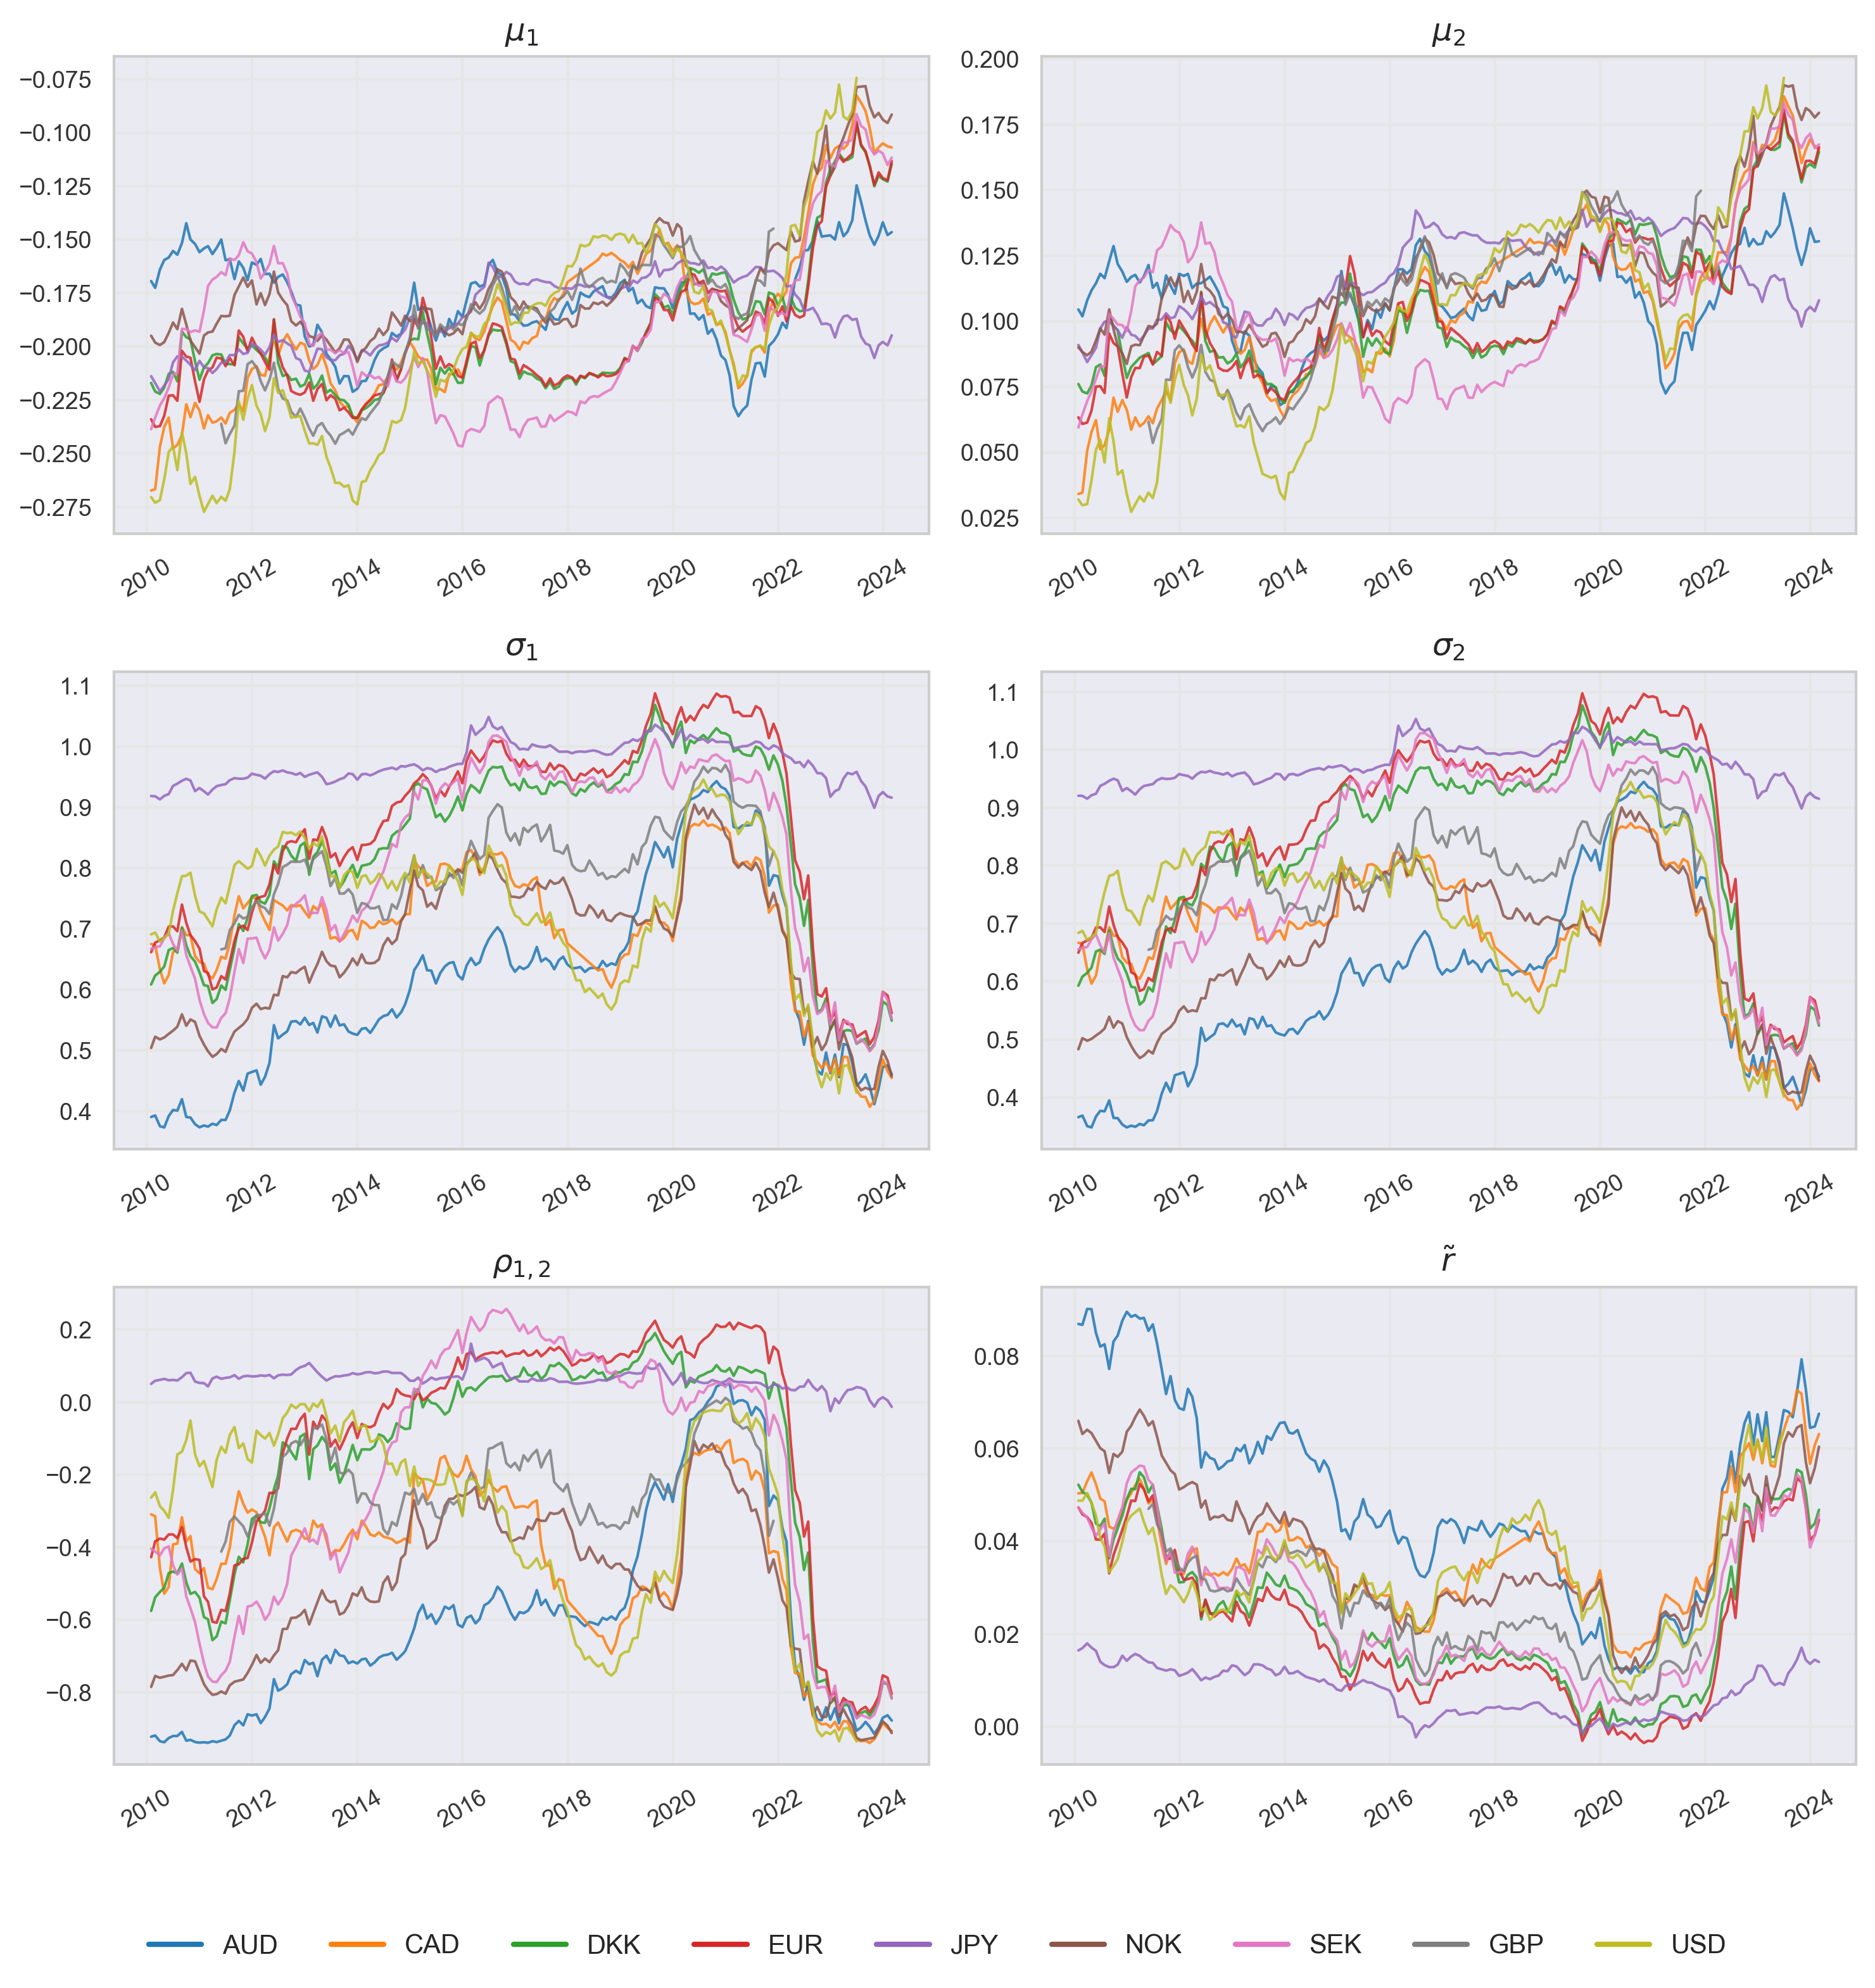
\includegraphics[width=\textwidth]{Figures/TrainingResults/dim2_baseline/ep5000/parameters/model_parameters_combined.png}
    \caption{Model-implied parameters for the baseline model with $\ell = 2$, evaluated over the full sample period 2010--2024. Each panel shows one implied parameter through time across all nine currencies, covering the drift, diffusion, correlation, and short-rate.}
    \label{fig:model_parameters_dim2}
\end{figure}



%--------------------------------------------------------
\section{Relation to Operator-Learning Theory}
\label{app:operator_learning_relation}
%--------------------------------------------------------


In Chapter~\ref{chap:model_comparison}, the decoder of the affine-inspired encoder--decoder framework is interpreted as a state-to-curve map and related to the operator-learning results of \citet{Benth2023} and \citet{Benth2024}. While the decoder does not fit directly within their theoretical setting, the connection is nonetheless relevant, as it speaks to whether the state-to-curve map is learnable in the sense established by these results. This section examines the relation more precisely by identifying where the two formulations align and where they differ.


\subsection{Operator-Learning Formulation of the Bond-Pricing Problem}


\citet{Benth2023} establish a universal approximation theorem for continuous maps between infinite-dimensioanl function spaces, generalising the classical result from $\mathbb{R}^n$ to settings where inputs are themselves functions rather than finite-dimensional vectors. Building on this framework, \citet{Benth2024} study the solution operator associated with a class of backward parabolic Cauchy problems in $\mathbb{R}^n$,
\begin{equation}
    \begin{cases}
        Lu + \partial_t u = f(x,t), & \text{in } \mathbb{R}^n \times [0,T) \\
        u(x,T) = \phi(x), & \text{in } \mathbb{R}^n,
    \end{cases}
\end{equation}
where $0 < T < \infty$ and
\begin{equation}
    Lu = \frac{1}{2} \sum_{i,j=1}^{n} a_{ij}(x,t)\partial^2_{ij} u 
       + \sum_{i=1}^{n} b_i(x,t)\partial_i u + c(x,t)u.
\end{equation}
where $\phi$ is the terminal condition and $f$ is the forcing term.

In their setting, the coefficients $a_{ij}$ and $b_i$ are held fixed, and the solution operator maps the terminal condition $\phi$, the zeroth-order coefficient $c$, and the forcing term $f$ to the corresponding solution function at a fixed time $t\in[0,T)$. This map may be written as 
\[
F_t:
(\phi,c,f)
\longmapsto
u(\cdot,t;\phi,c,f).
\]
Under the regularity conditions imposed by \citet{Benth2024}, $F_t$ is continuous as a map between function spaces, and therefore falls within the scope of \citet{Benth2023}, establishing that the solution operator admits a neural network approximation.

Under suitable regularity conditions, the no-arbitrage zero-coupon bond-pricing PDE considered in this thesis can be viewed as a special case of such a backward parabolic Cauchy problem. In the notation above, the terminal condition is $\phi \equiv 1$, the forcing term is $f=0$, and the zeroth-order coefficient is determined by the short-rate function $r$. The coefficients $a_{ij}$ and $b_i$ specify the diffusion and drift of the underlying state process respectively, and the solution $u$ corresponds to the bond price $P$.

Holding $a_{ij}, b_i, \phi$ and $f$ fixed, and allowing only the short-rate function $r$ to vary, the restricted bond-pricing solution operator may be written as 
\begin{equation}
    F^{\mathrm{bond}}_t: r\longmapsto P(\cdot\,,t;r),
    \label{eq:bondpricingOperatorBenth}
\end{equation}

where $P(x,t;r)$ denotes the bond-price function associated with the short rate specification $r$. The operator-learning formulation thus concerns how variation in the short rate function, as a function-valued input, changes the corresponding function-valued pricing solution.







\subsection{Relation to the Affine-Inspired Decoder}

In the framework of \citet{Benth2024}, the bond-pricing problem is formalised through the operator $F_t^{\text{bond}}$, whic maps a short rate specification to the corresponding dicount curve. In the setting of this thesis, the analagous pricing problem is represented by a different map. Let $\theta$ denote the learned parameters of the decoder. Once estimated, the decoder defines the state-to-curve map
\[
D_\theta:
\mathbb{R}^{\ell}
\longrightarrow
C([0,\tau_{\max}]),
\qquad
z
\longmapsto
P_\theta(z,\cdot),
\]
where \(P_\theta(z,\cdot)\) is the maturity-dependent bond-price curve generated from the latent state \(z\), and $C([0,\tau_{\text{max}}])$ denotes the space of continuous functions on $[0,\tau_{\text{max}}]$.



In contrast to the solution-operator formulation in \eqref{eq:bondpricingOperatorBenth}, the short-rate function is not an input to \(D_\theta\). Instead, it is determined internally by the learned map
\[
z
\longmapsto
\widetilde r_\theta(z).
\]
where $\tilde{r}_\theta(z)$ denotes the short rate implied by the latent state $z$ under the parameters $\theta$. The two maps therefore operate at different levels: $F_t^{\text{bond}}$ solves a pricing problems for each short-rate input and returns the corresponding curve, whereas $D_\theta$ evaluates a single learned function at varying latent states $z$, with parameters $\theta$ fixed after training. Consequently, \(D_\theta\) is not the solution operator analysed by \citet{Benth2024}.



Yet the operator-learning results of \citet{Benth2023} and \citet{Benth2024} provide a broader theoretical perspective on pricing solutions as learnable function-valued objects, even if they do not yield a direct approximation guarantee for the particular state-to-curve map $D_\theta$ studied in this thesis. 


%There is also a difference in how financial structure enters the approximation problem. In the affine-inspired encoder--decoder framework, the neural networks determine the model components entering the bond-pricing equation. For each latent state \(z\), the no-arbitrage ODE system is solved for the maturity-dependent coefficient paths \(A_z(\tau)\) and \(B_z(\tau)\), and bond prices are then obtained from
%\[
%P_\theta(z,\tau)
%=
%\exp\left(
%A_z(\tau)
%-
%B_z(\tau)\mathcal{G}_\theta(z,\tau)
%\right).
%\]
%The state-wise no-arbitrage structure imposed on the decoded curve therefore follows from the PDE-based construction of the decoder and the resulting ODE system. It is not a consequence of the operator-learning approximation result.

%The operator-learning results of \citet{Benth2023} and \citet{Benth2024} therefore provide a broader theoretical perspective for viewing pricing solutions as learnable function-valued objects. They do not, however, yield a direct approximation guarantee for the particular state-to-curve map \(D_\theta\) used in this thesis. The affine-inspired encoder--decoder remains a finite-dimensional latent-state model whose continuous bond-price curves are generated through its state-wise no-arbitrage pricing construction.